\documentclass[10pt,letterpaper]{article}
\usepackage[margin=0.70in,top=0.72in,bottom=0.68in,headheight=14pt,headsep=14pt]{geometry}
\usepackage[T1]{fontenc}
\usepackage{lmodern,microtype,parskip,enumitem,amssymb}
\usepackage{tabularx,booktabs,array,xcolor,graphicx}
\usepackage{tikz}
\usetikzlibrary{arrows.meta,positioning,calc}
\usepackage{listings,fancyhdr,hyperref}
\definecolor{navy}{HTML}{15384A}
\definecolor{teal}{HTML}{007D82}
\definecolor{pale}{HTML}{EDF5F5}
\definecolor{ink}{HTML}{273742}
\definecolor{muted}{HTML}{536773}
\definecolor{line}{HTML}{CCD8DD}
\definecolor{amber}{HTML}{926300}
\definecolor{green}{HTML}{206642}
\definecolor{red}{HTML}{9A3232}
\hypersetup{colorlinks=true,urlcolor=teal,linkcolor=teal,pdfauthor={USF AI in FinTech course},pdftitle={Project 0: Payment Rails Live - Technical Design and Cloud Supplement}}
\renewcommand{\familydefault}{\sfdefault}
\color{ink}
\setlength{\parindent}{0pt}
\setlength{\parskip}{5pt}
\setlength{\emergencystretch}{2em}
\setlist{nosep,leftmargin=16pt,topsep=5pt,itemsep=3pt}
\renewcommand{\arraystretch}{1.18}
\newcolumntype{Y}{>{\raggedright\arraybackslash}X}
\lstset{basicstyle=\ttfamily\fontsize{9}{11}\selectfont,columns=fullflexible,keepspaces=true,breaklines=true,showstringspaces=false,frame=single,rulecolor=\color{line},backgroundcolor=\color{pale},framesep=6pt,xleftmargin=6pt,xrightmargin=6pt,aboveskip=7pt,belowskip=7pt}
\pagestyle{fancy}\fancyhf{}
\fancyhead[L]{\fontsize{8.5}{10}\selectfont\color{muted}USF | AI in FinTech | Technical design and cloud supplement}
\fancyhead[R]{\fontsize{8.5}{10}\selectfont\color{muted}Project 0}
\fancyfoot[L]{\fontsize{8}{10}\selectfont\color{muted}Payment Rails Live | Fictional USD debit-card flow}
\fancyfoot[R]{\fontsize{8}{10}\selectfont\color{muted}\thepage\ / 20}
\renewcommand{\headrulewidth}{0.3pt}
\newcommand{\pagetitle}[2]{\noindent{\color{teal}\small\bfseries #1}\par\vspace{2pt}{\color{navy}\fontsize{21}{24}\selectfont\bfseries #2}\par\vspace{7pt}}
\newcommand{\smalltitle}[1]{\par\vspace{5pt}{\color{navy}\large\bfseries #1}\par\vspace{2pt}}
\newcommand{\screen}[2]{\begin{center}\IfFileExists{../screenshots/#1}{\includegraphics[width=\linewidth,height=#2,keepaspectratio]{../screenshots/#1}}{\fcolorbox{line}{pale}{\parbox[c][#2][c]{0.94\linewidth}{\centering\textbf{Screenshot asset: #1}\par The full distribution includes the captured running dashboard in the screenshots folder. A standalone editor preview can omit external image assets.}}}\end{center}}
\begin{document}
\pagetitle{01 / TECHNICAL DESIGN}{A small, observable payment system}
\smalltitle{Purpose and success criteria}
Project 0 implements the six-participant payment rail as independent local Python processes. Its audience is an instructor-led FinTech class. A learner should be able to locate the payment decision, explain a hold, distinguish capture from clearing and settlement, and prove that replay does not create a second financial effect.

A single command must start the six processes and browser dashboard. All runtime logic uses the Python standard library, fictional accounts, and deterministic rules. The same package can run in a container on one cloud VM. Independent cloud services are a future generation path, not delivered infrastructure.

\begin{tabularx}{\linewidth}{>{\raggedright\arraybackslash}p{4.3cm}Y}
\toprule
\textbf{Required observable result} & \textbf{Evidence} \\ \midrule
Real participant boundary & Six child PIDs; role-specific state and received/returned messages. \\
Complete authorization path & Forward request to issuer, then reverse response to payer. \\
Financial-stage distinction & Hold at approval; capture marker; debit/obligation at clearing; proceeds and fee allocations at settlement. \\
Safe repeat behavior & Stable payment/operation IDs, recorded outcomes, no second debit or credit. \\
Useful failures & Valid decline reasons, input/transition errors, and worker failure requiring Reset. \\
Teaching portability & README, launchers, editable diagrams, fixtures, tests, screenshots, documents, manifest, and ZIP. \\
\bottomrule
\end{tabularx}

\smalltitle{Implementation boundaries}
The server hosts one shared instructor session. Financial state is in memory and belongs to the participant that handles it. Refreshing a browser does not start a new bank session. Reset or restart does.

The application models a full-capture USD debit-card purchase. It has no real payment credentials, real bank connections, LLM decisions, merchant identity verification, EMV cryptograms, 3-D Secure, refunds, chargebacks, partial captures, authorization expiry, or durable recovery. It does not implement ISO 8583 or official Visa/Mastercard wire formats.

\begin{quote}\textbf{Two teaching conventions}\par
The code posts the payer debit at clearing and separates settlement into another visible stage. Real financial posting and settlement timing depend on products, issuers, networks, and processing arrangements. Its fee rates are illustrative, not market quotations.\end{quote}

\smalltitle{Reader map}
Pages 2--10 explain processes, contracts, financial state, and verification. Pages 11--18 give local container and cloud VM runbooks. Pages 19--20 describe the future distributed design and authoritative sources. The companion guide provides the classroom narration.

\clearpage
\pagetitle{02 / TECHNICAL DESIGN}{Runtime architecture and ownership}
\begin{center}
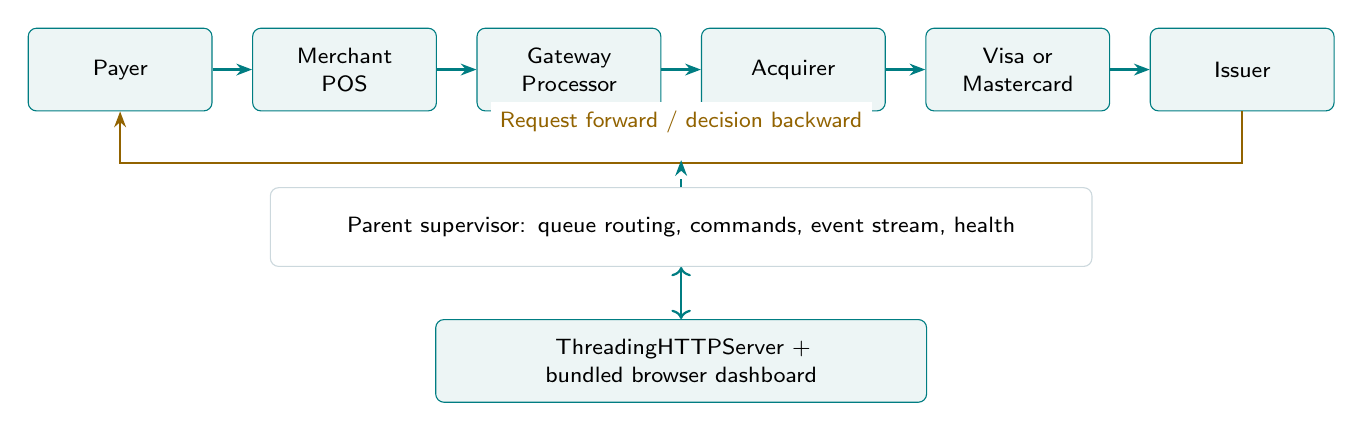
\begin{tikzpicture}[font=\fontsize{8.5}{10}\selectfont,box/.style={draw=teal,fill=pale,rounded corners=3pt,align=center,text width=2.1cm,minimum height=1.05cm},arr/.style={-{Stealth[length=2mm]},thick,teal}]
\foreach \name/\label/\x in {p/Payer/0,m/{Merchant\\POS}/2.85,g/{Gateway\\Processor}/5.7,a/Acquirer/8.55,n/{Visa or\\Mastercard}/11.4,i/Issuer/14.25}{\node[box] (\name) at (\x,0) {\label};}
\draw[arr] (p)--(m);\draw[arr] (m)--(g);\draw[arr] (g)--(a);\draw[arr] (a)--(n);\draw[arr] (n)--(i);
\draw[arr,amber] (i.south)--++(0,-0.65)-|(p.south);
\node[fill=white,text=amber] at (7.125,-0.67) {Request forward / decision backward};
\node[draw=line,fill=white,align=center,text width=10.2cm,rounded corners=3pt,minimum height=1.0cm] (s) at (7.125,-2) {Parent supervisor: queue routing, commands, event stream, health};
\draw[arr,dashed] (s)--(7.125,-1.15);
\node[box,text width=6cm] (w) at (7.125,-3.7) {ThreadingHTTPServer + bundled browser dashboard};
\draw[arr,<->] (s)--(w);
\end{tikzpicture}
\end{center}

\begin{tabularx}{\linewidth}{>{\raggedright\arraybackslash}p{3.2cm}Y}
\toprule
\textbf{Process} & \textbf{Owns / does} \\ \midrule
Payer & Purchase initiation and returned receipt/outcome. Authoritative funds come from issuer observations. \\
Merchant & Payment records, authorization outcomes, full-capture intent, and batch membership. \\
Gateway & Contract checks, request identity, and processor routing. \\
Acquirer & Authorized/cleared records, merchant proceeds, and illustrative fee recipient buckets. \\
Network & Brand routing and membership/amount reconciliation; no fee ledger. \\
Issuer & Account status, posted balances, holds, and unsettled obligations. \\
Supervisor & Child lifecycle, inbox delivery order, pacing, commands, and observed state snapshots. \\
\bottomrule
\end{tabularx}

Use the spawn multiprocessing context for portability. Each child is created from an importable role module; the guarded launch entry point avoids recursively spawning on Windows. Inbox/outbox messages are serializable dictionaries. One supervisor command lock coordinates instructor commands and automatic advancement.

An event is recorded only when the process receives/handles a message or the supervisor observes an explicit runtime/control event. Animation reads that evidence. Observed snapshots may be temporarily between stages while a response is pending.

\clearpage
\pagetitle{03 / TECHNICAL DESIGN}{Messages and identities}
\smalltitle{Shared message envelope}
Every business message carries payment/operation identity and routing information. The JSON trace exposes the actual envelopes; the fields below form the teaching contract. Batch operations carry their batch ID and member records alongside the envelope.

\begin{tabularx}{\linewidth}{>{\raggedright\arraybackslash}p{4.0cm}>{\raggedright\arraybackslash}p{3.0cm}Y}
\toprule
\textbf{Field} & \textbf{Type} & \textbf{Meaning} \\ \midrule
payment\_id & String & Stable transaction identity; batch messages identify their members. \\
operation\_id & String & Stable identity of authorize/capture/clear/settle operation. \\
sender / recipient & Role strings & Current hop; change as the message travels. \\
type & String & Request or response and financial stage. \\
amount\_cents & Integer & Exact USD cents; no binary floating-point money. \\
currency & String & USD only. \\
account\_id / token & Synthetic string & Fixture reference, never a card number. \\
network & String & Visa or Mastercard in the simulation. \\
outcome / reason & String or null & Recorded result and readable reason. \\
session / routing data & Metadata & Run isolation, original payload, route/stage information. \\
\bottomrule
\end{tabularx}

\smalltitle{Input policy}
Amounts must be true integers from 100 through 1000000 cents (\$1--\$10,000). Booleans, strings, floats, zero, negative amounts, and other currencies are invalid. IDs are nonempty strings of at most 100 characters. Known synthetic account IDs must match a fixture. A valid but inactive account produces a decline; an unknown account is not approved.

\smalltitle{Idempotency and conflict}
Participants remember a canonical payload and its result by the pair (operation ID, message type). Re-delivering the same operation with the same financial details returns the original result. Reusing an ID with different amount, account, currency, brand, stage, or batch membership is a conflict. Transport-only sender/recipient changes do not redefine the payment.

The fixture accounts are demo-active (50000 cents), demo-low (1000 cents), and demo-inactive (50000 cents, inactive). The invalid preset uses an unknown synthetic token. A payment ID identifies one purchase across stages. An operation ID identifies one attempted action on that purchase. An authorization ID cannot be reused to capture. A retry must retain its original ID rather than allocate a fresh financial operation.

\smalltitle{Trace versus storage}
The trace is an instructor-visible audit of this run, not a durable accounting log. Download it before Reset if it is useful for discussion. A future implementation must persist idempotency records and financial updates in the same transaction.

\clearpage
\pagetitle{04 / TECHNICAL DESIGN}{Authorization is a round trip}
\begin{center}
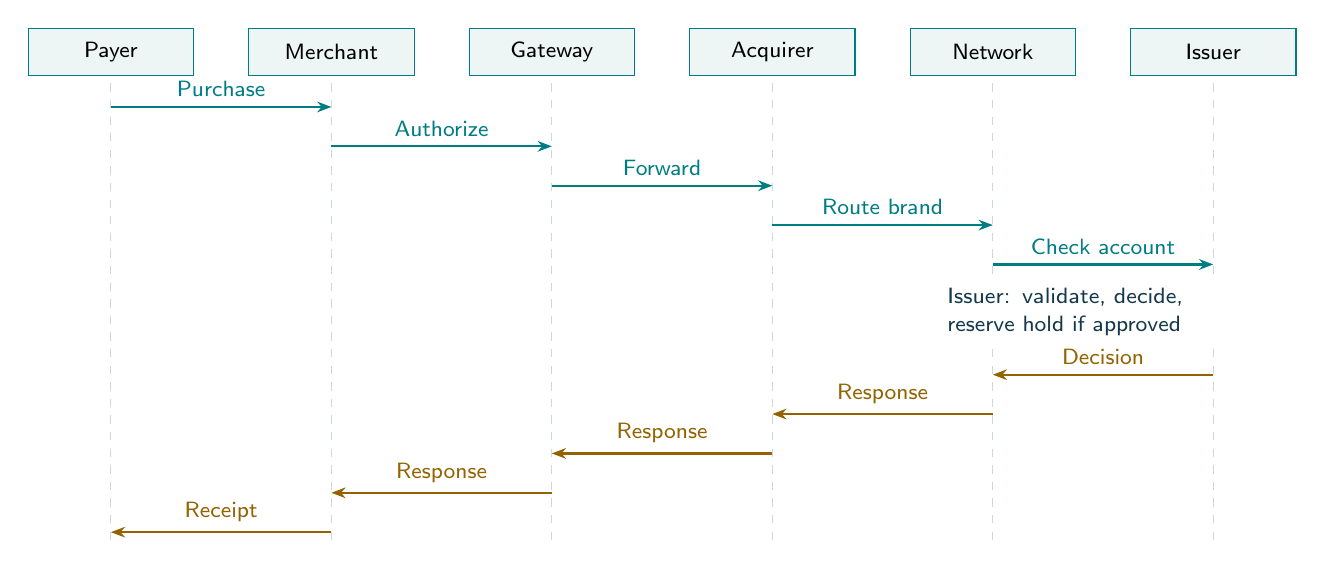
\begin{tikzpicture}[x=1cm,y=1cm,font=\fontsize{8}{10}\selectfont,arr/.style={-{Stealth[length=1.8mm]},teal,thick}]
\foreach \name/\label/\x in {p/Payer/0,m/Merchant/2.8,g/Gateway/5.6,a/Acquirer/8.4,n/Network/11.2,i/Issuer/14}{\node[draw=teal,fill=pale,minimum width=2.1cm,minimum height=.6cm] at (\x,0) {\label};\draw[dashed,line] (\x,-.4)--(\x,-6.3);}
\draw[arr] (0,-.7)--node[above]{Purchase}(2.8,-.7);
\draw[arr] (2.8,-1.2)--node[above]{Authorize}(5.6,-1.2);
\draw[arr] (5.6,-1.7)--node[above]{Forward}(8.4,-1.7);
\draw[arr] (8.4,-2.2)--node[above]{Route brand}(11.2,-2.2);
\draw[arr] (11.2,-2.7)--node[above]{Check account}(14,-2.7);
\node[anchor=west,text width=3.4cm,fill=white,text=navy] at (10.5,-3.3) {Issuer: validate, decide, reserve hold if approved};
\draw[arr,amber] (14,-4.1)--node[above]{Decision}(11.2,-4.1);
\draw[arr,amber] (11.2,-4.6)--node[above]{Response}(8.4,-4.6);
\draw[arr,amber] (8.4,-5.1)--node[above]{Response}(5.6,-5.1);
\draw[arr,amber] (5.6,-5.6)--node[above]{Response}(2.8,-5.6);
\draw[arr,amber] (2.8,-6.1)--node[above]{Receipt}(0,-6.1);
\end{tikzpicture}
\end{center}

\smalltitle{Issuer decision order}
Validate the account and active status, then compare the request with current available funds. Available equals posted balance less active holds. Each issuer process handles one inbox message at a time, so competing authorizations share the latest hold state.

For a \$50 authorization from a \$500 opening account, record a \$50 hold and approval. Keep posted balance at \$500; available becomes \$450. If funds are insufficient, return a decline with no hold. An inactive account has a different reason, allowing the instructor to compare business failures.

\smalltitle{When the POS may show the decision}
The issuer's decision exists when it handles the request, but the merchant and payer only learn it when the reverse messages reach them. The dashboard makes these moments separate. Do not equate a request being enqueued with a response arriving.

\smalltitle{The decline still returns}
A valid issuer decline follows the complete reverse path. Earlier contract errors can be returned by the gateway. A process crash is observed as a failure and pauses the run; it must not be turned into a fabricated issuer decline or approval.

\clearpage
\pagetitle{05 / TECHNICAL DESIGN}{Capture, clearing, and settlement}
\begin{center}
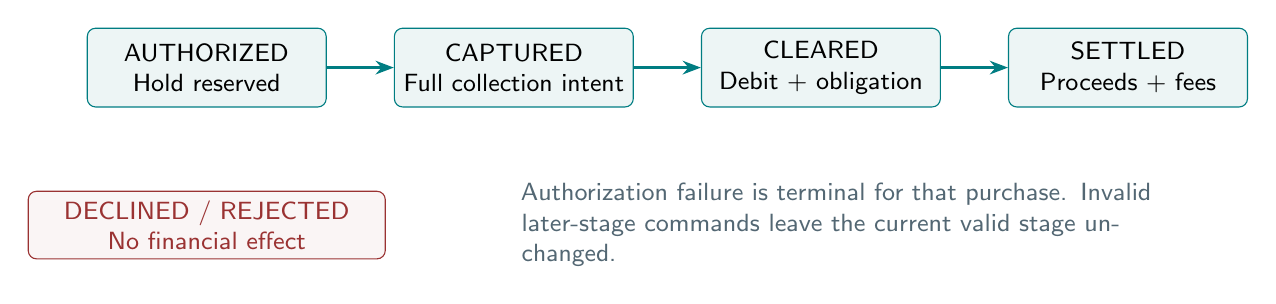
\begin{tikzpicture}[font=\fontsize{9}{11}\selectfont,box/.style={draw=teal,fill=pale,rounded corners=3pt,align=center,text width=2.8cm,minimum height=1.0cm},arr/.style={-{Stealth},thick,teal}]
\node[box] (a) at (0,0) {AUTHORIZED\\Hold reserved};
\node[box] (b) at (3.9,0) {CAPTURED\\Full collection intent};
\node[box] (c) at (7.8,0) {CLEARED\\Debit + obligation};
\node[box] (d) at (11.7,0) {SETTLED\\Proceeds + fees};
\draw[arr] (a)--(b);\draw[arr] (b)--(c);\draw[arr] (c)--(d);
\node[draw=red,fill=red!5,text=red,rounded corners=3pt,align=center,text width=4.3cm] (e) at (0,-2) {DECLINED / REJECTED\\No financial effect};
\node[align=left,text width=8cm,text=muted] at (8,-2) {Authorization failure is terminal for that purchase. Invalid later-stage commands leave the current valid stage unchanged.};
\end{tikzpicture}
\end{center}

\begin{tabularx}{\linewidth}{>{\raggedright\arraybackslash}p{3cm}Y}
\toprule
\textbf{Operation} & \textbf{Required state and effect} \\ \midrule
Capture & An approved authorization exists. Record full amount only. Keep the hold and posted balance unchanged. \\
Clear & Captured members exist and reconcile. Release each hold, post the gross debit once, record a gross settlement obligation. \\
Settle & A cleared, reconciled batch exists. Remove its obligation once and credit merchant proceeds plus fee allocations once. \\
Replay & Return the recorded operation outcome. Preserve financial state and original operation identity. \\
\bottomrule
\end{tabularx}

\smalltitle{No implicit stage jump}
A capture request before authorization is invalid. A settlement request before clearing is invalid. A payment cannot be included in two independently credited settlement batches. Capture remains local to the merchant; the issuer hold stays unchanged until clearing. Guided controls enqueue stage work; Next Message delivers the resulting hops. A stage is complete only after its recorded response.

\smalltitle{The difference between accounts and obligations}
The payer's posted balance represents fictional deposit funds. A hold is a reservation against those funds. A cleared obligation says the issuer owes the cleared sale amount to the merchant side. It is tracked separately so the dashboard can show the period between payer debit and merchant proceeds.

The program uses compact role-local state rather than a production double-entry ledger. It checks cent arithmetic and batch reconciliation, but it does not implement a bank general ledger, liquidity management, or legal settlement finality.

\smalltitle{Reading the event history}
Request events, handled events, state snapshots, and returned outcomes show intermediate steps. They may reveal an issuer-cleared payment before the merchant sees the final acknowledgement. This lag is a useful part of the lesson. The dashboard's Awaiting settlement includes issuer obligations plus funding in the settlement return path until the acquirer records the merchant credit. It can show SETTLING during that interval; the issuer's own pending ledger remains separate.

\clearpage
\pagetitle{06 / TECHNICAL DESIGN}{Integer-cent financial arithmetic}
\smalltitle{Exact fee function}
Let \(a\) be gross cents and \(b\) a rate in basis points. The implementation rounds a nonnegative fee half up:
\[
\mathrm{rateFee}(a,b)=\left\lfloor\frac{a b + 5000}{10000}\right\rfloor.
\]
Interchange uses 200 basis points; network fee uses 10; processing/acquiring uses 20 plus a fixed 10 cents. Compute and round each percentage component separately. Merchant proceeds equal gross minus the three complete components.

\begin{tabularx}{\linewidth}{Yrrr}
\toprule
\textbf{Amount} & \textbf{\$1.00} & \textbf{\$12.34} & \textbf{\$50.00} \\ \midrule
Gross cents & 100 & 1234 & 5000 \\
Interchange cents & 2 & 25 & 100 \\
Network cents & 0 & 1 & 5 \\
Acquirer/processor cents & 10 & 12 & 20 \\
Total fees cents & 12 & 38 & 125 \\
Merchant proceeds cents & 88 & 1196 & 4875 \\
\bottomrule
\end{tabularx}

\smalltitle{State of the approved example}
\begin{tabularx}{\linewidth}{Yrrrr}
\toprule
\textbf{Stage} & \textbf{Posted} & \textbf{Held} & \textbf{Available} & \textbf{Obligation} \\ \midrule
Initial & 50000 & 0 & 50000 & 0 \\
Authorized & 50000 & 5000 & 45000 & 0 \\
Captured & 50000 & 5000 & 45000 & 0 \\
Cleared & 45000 & 0 & 45000 & 5000 \\
Settled & 45000 & 0 & 45000 & 0 \\
\bottomrule
\end{tabularx}
All values in this table are cents. At settlement, merchant 4875 + issuer 100 + network 5 + acquirer/processor 20 = 5000. Settling the same operation again must leave all four allocations unchanged.

\smalltitle{Why round components independently?}
A fractional-cent fee cannot be displayed as a posted cent balance. Rounding the aggregate percentage once can differ from rounding three recipient components. The displayed allocation totals are sums of already-rounded per-payment components, never a fresh calculation on the batch gross. All fee recipient buckets are recorded in the acquirer's illustrative payout ledger, not separate issuer/network deposit accounts.

\smalltitle{Validation and teaching limits}
Purchases below 100 cents are outside the toy input policy. Fee functions may still be unit-tested at small values to exercise rounding boundaries. A configured total fee cannot exceed gross. Real pricing uses product, merchant, country, and network-specific rules; these fixed rates are classroom constants.

\clearpage
\pagetitle{07 / TECHNICAL DESIGN}{Batches reconcile before settlement}
\smalltitle{A batch is a named set of captured payments}
A clearing batch retains member payment IDs, gross amounts, currency, account/merchant/brand identity, and a digest of that membership. The merchant validates captured eligibility; acquirer, network, and issuer check their corresponding records before accepting the stage. Fee components are derived from recorded amounts using the fixed policy.

\begin{enumerate}
\item Select eligible captured payments once. Preserve a batch ID and membership across the operation's hops.
\item Reject missing, extra, duplicate, previously processed, or wrong-stage members.
\item Match each member's amount/currency against the participant's stored original payment.
\item Match gross against the sum of member amounts and recompute the membership digest. The acquirer derives each fee allocation from the unchanged member amounts.
\item Clear each eligible member at the issuer: release its hold, debit gross once, record the obligation.
\item Settle only the corresponding cleared batch. Record each allocation and remove each obligation once.
\end{enumerate}

\smalltitle{A two-payment reconciliation example}
\begin{tabularx}{\linewidth}{Yrrrr}
\toprule
\textbf{Member} & \textbf{Gross} & \textbf{Fees} & \textbf{Merchant} & \textbf{Stage} \\ \midrule
P0001 & 5000 & 125 & 4875 & Captured \\
P0002 & 1234 & 38 & 1196 & Captured \\
Batch total & 6234 & 163 & 6071 & Eligible \\
\bottomrule
\end{tabularx}
A payload claiming gross 6235 is inconsistent even if the membership looks right. A payload replacing P0002 with an unknown ID is inconsistent even if gross remains 6234. Both kinds of mismatch require rejection before marking settlement successful.

\smalltitle{Retry versus a different batch}
A replay uses the same operation ID, batch identity, and members; its recorded result is returned. Changed membership under that ID is a conflict. A new ID cannot make an already-settled payment eligible again. These protections are related but distinct: operation history handles retries; payment stage and membership checks protect against new operations on old funds.

\smalltitle{Distributed failure is intentionally visible}
The local toy sequences the participant hops. It does not provide a distributed commit protocol. If a participant fails after another has changed local state, the run pauses and requires Reset. It must not claim recovered or atomic cross-process settlement. A future transactional inbox/outbox and durable ledger are necessary for recovery.

\smalltitle{Useful verification evidence}
Export the trace, inspect each batch member, compare totals, and check allocations after the reverse response finishes. Unit tests alter membership and totals; integration tests exercise the complete accepted and rejected batch paths.

\clearpage
\pagetitle{08 / TECHNICAL DESIGN}{Local browser and JSON interfaces}
The browser uses relative URLs against the Python HTTP server. It polls for observations and submits commands. The interface is intended for the local shared instructor session.

\begin{tabularx}{\linewidth}{>{\raggedright\arraybackslash}p{5.0cm}Y}
\toprule
\textbf{Route} & \textbf{Purpose} \\ \midrule
GET /api/state?after=N & Current actor/payment/financial state plus events after sequence N. Initial request uses zero. \\
POST /api/command & JSON command body with an action and its relevant fields. \\
GET /api/trace & Download the current run's full observed JSON trace. \\
GET /healthz & Server and participant health evidence. \\
GET / & Bundled dashboard; static CSS/JS served by the same process. \\
\bottomrule
\end{tabularx}

\begin{tabularx}{\linewidth}{>{\raggedright\arraybackslash}p{2.5cm}Y}
\toprule
\textbf{Action} & \textbf{Relevant fields / behavior} \\ \midrule
purchase & preset: approved, insufficient, inactive, invalid; optional amount\_cents, account\_id, network. \\
step & Deliver the next pending message in Guided mode. \\
capture & payment\_id of an authorized payment; full amount only. \\
clear / settle & Optional batch\_id; clear selects captured members; settle selects the oldest cleared batch when omitted. \\
mode & mode: guided or automatic. \\
pause & paused: true or false; stop/resume automatic advancement. \\
speed & speed\_ms: integer automatic delivery interval, 150--1500 ms. \\
reset & seed: optional integer 0--2147483647; default 7; replace workers and state. \\
replay & payment\_id: resend the recorded authorization operation. \\
\bottomrule
\end{tabularx}

\smalltitle{Try a local command after starting the server}
\begin{lstlisting}
curl -s http://127.0.0.1:8010/healthz
curl -s -X POST http://127.0.0.1:8010/api/command \
  -H 'Content-Type: application/json' \
  -d '{"action":"purchase","preset":"approved"}'
curl -s http://127.0.0.1:8010/api/state?after=0
\end{lstlisting}
A command response means the action was accepted or rejected by the supervisor. Financial completion is observed through subsequent participant events and state. API input errors return explicit errors rather than a browser-only validation rule.

\smalltitle{Session and event cursor}
Reset starts a fresh session and trace. A client detects the changed session and replaces its selected transaction and event cursor. Late events from the old session must not contaminate the new balances. This API is not a multi-user payment service.

\clearpage
\pagetitle{09 / TECHNICAL DESIGN}{Pacing, process health, and reset}
\smalltitle{Guided mode}
The supervisor holds outbound business messages until the instructor requests Next Message. It delivers one queued hop, waits for the role's response event, records any resulting messages/snapshot, then makes the next hop available. The browser highlights the received hop and provides its explanation.

Capture, Clear Batch, and Settle Batch enqueue stage operations. They do not skip the transport or immediately assign finished balances in the dashboard. Controls show pending work so the instructor knows when to step.

\smalltitle{Automatic mode}
A seeded generator produces fictional POS purchases, including approvals and declines. The supervisor advances messages at the selected interval and schedules capture/clearing/settlement for eligible records. Accelerated batches represent later stages within a classroom timescale; they are not a statement of real clearing time.

Reset with the same seed repeats the generated purchase data. Event wall-clock times and process IDs vary. Pause freezes automatic input and delivery; the trace remains inspectable. Speed changes pacing, not payment rules.

\smalltitle{Process failure}
Track running child PIDs and exit codes. If a process exits unexpectedly or fails to answer a delivery, show the observed failure, pause further financial work, and require Reset. Preserve whatever state is actually observed. Do not infer an approval, rollback, or settlement acknowledgement that no participant emitted.

\smalltitle{Reset and shutdown}
\begin{enumerate}
\item Suspend automatic advancement and serialize the reset with command handling.
\item Stop all old workers, join them, and close their queues.
\item Allocate a fresh run/session, queues, participant fixtures, and random generator.
\item Spawn six new workers and verify startup responses.
\item Replace observable state and clear old pending messages/cursors.
\end{enumerate}
Ctrl+C and termination signals stop the server and workers. The server is bound to loopback by default. The container explicitly binds within its own network namespace and is published only to host loopback.

\smalltitle{Shared-session behavior}
Two browser tabs see one supervisor. A reset from one tab resets both views when they next poll. The design supports an instructor presentation, not concurrent independent student accounts. A multi-session extension requires separate actor sets or explicit durable session partitioning.

\clearpage
\pagetitle{10 / TECHNICAL DESIGN}{Acceptance and browser verification}
\begin{tabularx}{\linewidth}{>{\raggedright\arraybackslash}p{3.8cm}Y}
\toprule
\textbf{Case group} & \textbf{Required evidence} \\ \midrule
Approval & Complete forward/reverse path; one hold; no posted debit before clearing. \\
Declines & Insufficient funds, inactive account, unknown account; reasons visible; no new hold. \\
Input contract & Reject float/string/bool amounts, unsupported currency/brand, bounds, missing/overlong IDs. \\
Replay/conflict & Matching retry returns recorded result; changed details under ID rejected; balances unchanged. \\
Stage ordering & Capture before approval, clear before capture, settle before clearing rejected. \\
Competing authorizations & Combined holds cannot exceed available funds; later request sees earlier reservations. \\
Clearing/settlement & Debit once; release hold once; obligation tracked then removed; credit each allocation once. \\
Fees and batches & Half-up boundaries; sum rounded members; mismatch membership/total rejected. \\
Runtime isolation & Same seed repeats input; Reset replaces six PIDs and ignores old events; shutdown leaves no child alive. \\
\bottomrule
\end{tabularx}

\smalltitle{Run the delivered checks}
From the project root:
\begin{lstlisting}
python3 -m unittest discover -s tests -v
python3 start.py --no-browser
\end{lstlisting}
Use the project's verification record for the checks actually run on the delivery machine. A test list in this document is an acceptance specification; it is not evidence that an unavailable platform or cloud deployment was tested.

\smalltitle{Browser acceptance}
\begin{itemize}
\item Check the page loads, six participant labels/PIDs appear, and there are no console errors.
\item Step an authorization; compare highlighted sender/recipient with trace ordering and returned decision.
\item Run approval through settlement; compare financial panels with the cent values on page 6.
\item Verify scenario selection, transaction/message selection, pause, speed, reset, and trace download.
\item Use keyboard focus and shortcuts. With reduced motion, confirm animations stop but highlights/events remain readable.
\item Verify a failed worker pauses the demonstration and offers Reset.
\end{itemize}

\smalltitle{Document and package verification}
Compile both sources, confirm the course guide has exactly ten pages, render every PDF page, and inspect for clipping/overlap. Final exported PDFs must contain the actual screenshot files. Verify the manifest/ZIP includes source and fixtures rather than just PDFs. Container verification has a separate gate on page 11.

\clearpage
\pagetitle{11 / CLOUD SUPPLEMENT}{Stage 1: the working local container}
\smalltitle{Prerequisites and image}
Install a working Docker Engine or Docker Desktop. Start its engine and run \texttt{docker version}. The supplied Dockerfile uses Python 3.13 slim, copies the stdlib implementation and bundled dashboard, runs as a non-root user, and starts the server on container port 8010. There is no pip installation.

From the project root on macOS/Linux (Windows can use the same Docker arguments):
\begin{lstlisting}
docker build -t payment-rails-live:project0 .
docker run --name payment-rails-live --init --rm \
  -p 127.0.0.1:8010:8010 payment-rails-live:project0
\end{lstlisting}
Open \url{http://127.0.0.1:8010}. Host loopback publishing makes the dashboard available on your machine. Inside the container the server binds to 0.0.0.0 so Docker can forward that local host port.

\smalltitle{Smoke-test gate}
In a second terminal:
\begin{lstlisting}
curl -fsS http://127.0.0.1:8010/healthz
docker logs payment-rails-live
python3 qa/smoke_http.py http://127.0.0.1:8010
\end{lstlisting}
Confirm six running actors. Create an approved purchase and step through capture, clearing, and settlement in the browser. Compare \$48.75 proceeds and \$1.25 fees. Stop with Ctrl+C or \texttt{docker stop payment-rails-live}; check the container exits and the local port closes.

\smalltitle{Match the target VM architecture}
The runbooks below choose x86/amd64 VMs. If building on an Apple Silicon laptop, build an amd64 image explicitly before exporting:
\begin{lstlisting}
docker build --platform linux/amd64 \
  -t payment-rails-live:project0 .
docker save -o payment-rails-project0.tar \
  payment-rails-live:project0
\end{lstlisting}
Use a working emulation/buildx installation or an amd64 build machine if cross-building is unavailable. Alternatively choose an arm64 VM and matching image intentionally. An image archive avoids a container registry dependency in the classroom route.

\smalltitle{Delivery status versus instructions}
These commands are executable instructions. Consult \texttt{TEST\_REPORT.md and VERIFICATION.json} for whether Docker ran on the delivery machine; a missing daemon is recorded as unavailable rather than a passed smoke test. No cloud resource is created by building this package.

\clearpage
\pagetitle{12 / CLOUD SUPPLEMENT}{Common VM procedure and gates}
\smalltitle{Stages 2 and 3 are different}
Stage 2 runs the unchanged six-process container on one Ubuntu VM. Only SSH is permitted through the VM's public network boundary; the dashboard remains on remote host loopback and is reached through a tunnel. Stage 3 would deploy participants separately and replace queues/state, described on page 19.

Cloud commands in pages 13--18 are examples for an instructor to execute in a dedicated account/project/resource group. They provision billable resources. Fill every configuration input before executing, verify permissions, and tear down after class. These resources have not been provisioned as part of Project 0.

\smalltitle{Install Docker on the fresh Ubuntu VM}
The cloud pages tell you how to connect. On that VM, install from Docker's official repository. These commands use Ubuntu 24.04 or 22.04 as selected by the provider runbook:
\begin{lstlisting}
sudo apt-get update
sudo apt-get install -y ca-certificates curl
sudo install -m 0755 -d /etc/apt/keyrings
sudo curl -fsSL https://download.docker.com/linux/ubuntu/gpg \
  -o /etc/apt/keyrings/docker.asc
sudo chmod a+r /etc/apt/keyrings/docker.asc
P0_CODENAME=$(. /etc/os-release; printf '%s' "$VERSION_CODENAME")
P0_ARCH=$(dpkg --print-architecture)
printf '%s\n' \
  'Types: deb' \
  'URIs: https://download.docker.com/linux/ubuntu' \
  "Suites: $P0_CODENAME" \
  'Components: stable' \
  "Architectures: $P0_ARCH" \
  'Signed-By: /etc/apt/keyrings/docker.asc' | \
  sudo tee /etc/apt/sources.list.d/docker.sources
sudo apt-get update
sudo apt-get install -y docker-ce docker-ce-cli containerd.io
sudo systemctl enable --now docker
sudo docker run --rm hello-world
\end{lstlisting}
Source: \href{https://docs.docker.com/engine/install/ubuntu/}{Docker Engine installation on Ubuntu}. The repository setup is adapted to avoid a convenience-script dependency. The fresh VM has no conflicting prior Docker packages.

\smalltitle{Load and start the transferred image on the VM}
\begin{lstlisting}
sudo docker load -i payment-rails-project0.tar
sudo docker run -d --name payment-rails-live --init \
  -p 127.0.0.1:8010:8010 payment-rails-live:project0
curl -fsS http://127.0.0.1:8010/healthz
\end{lstlisting}
Require six running actors, a successful local health response, and a passed browser \$50 scenario through the tunnel. Stop with \texttt{sudo docker stop payment-rails-live}, then \texttt{sudo docker rm payment-rails-live}. Restart starts fresh memory; export the trace before stopping if needed.

\clearpage
\pagetitle{13 / CLOUD SUPPLEMENT}{AWS Lightsail: create the classroom VM}
\smalltitle{Prerequisites and configuration}
Use AWS CLI v2, an authenticated profile with Lightsail create/manage permissions, a supported Region/Availability Zone, and a budget for one Linux VM. Use a dedicated instance/key name. The SSH client and local amd64 image archive must be ready. Set \texttt{P0\_CIDR} to your current public IPv4 plus /32.

\begin{lstlisting}
P0_REGION=us-east-1
P0_AZ=us-east-1a
P0_NAME=payment-rails-project0
P0_KEYNAME=payment-rails-project0-key
P0_KEY="$PWD/payment-rails-project0.pem"
P0_CIDR=YOUR_PUBLIC_IPV4/32
aws sts get-caller-identity
aws lightsail get-blueprints --region "$P0_REGION" \
  --query "blueprints[?isActive==\`true\` && group=='ubuntu'].{id:blueprintId,version:version}" \
  --output table
aws lightsail get-bundles --region "$P0_REGION" \
  --query 'bundles[?isActive==`true` && ramSizeInGb==`2`].{id:bundleId,platform:supportedPlatforms,price:price}' \
  --output table
\end{lstlisting}
Choose the active Ubuntu 24.04 blueprint ID and a Linux 2 GB bundle ID returned in that Region; do not assume old IDs stay active. Enter those actual results:
\begin{lstlisting}
P0_BLUEPRINT=ACTIVE_UBUNTU_24_BLUEPRINT_ID
P0_BUNDLE=ACTIVE_LINUX_2GB_BUNDLE_ID
aws lightsail create-key-pair --region "$P0_REGION" \
  --key-pair-name "$P0_KEYNAME" \
  --query privateKeyBase64 --output text > "$P0_KEY"
chmod 600 "$P0_KEY"
aws lightsail create-instances --region "$P0_REGION" \
  --instance-names "$P0_NAME" --availability-zone "$P0_AZ" \
  --blueprint-id "$P0_BLUEPRINT" --bundle-id "$P0_BUNDLE" \
  --key-pair-name "$P0_KEYNAME" --ip-address-type ipv4
aws lightsail put-instance-public-ports --region "$P0_REGION" \
  --instance-name "$P0_NAME" \
  --port-infos "fromPort=22,toPort=22,protocol=tcp,cidrs=$P0_CIDR"
\end{lstlisting}
Wait for the instance to exist before setting ports. This replaces the public port list with SSH from the instructor's IPv4; no dashboard port is opened.

\smalltitle{Gate before moving the image}
\begin{lstlisting}
aws lightsail get-instance --region "$P0_REGION" \
  --instance-name "$P0_NAME" \
  --query 'instance.{state:state.name,ip:publicIpAddress,user:username}'
\end{lstlisting}
Wait for running, record public IP and username, and confirm the firewall contains only the intended SSH rule. For an Ubuntu blueprint the expected user is ubuntu; use the actual returned username if it differs.

Sources: \href{https://docs.aws.amazon.com/lightsail/latest/userguide/getstarted-awscli.html}{Lightsail CLI guide}, \href{https://docs.aws.amazon.com/cli/latest/reference/lightsail/get-blueprints.html}{blueprints}, \href{https://docs.aws.amazon.com/cli/latest/reference/lightsail/get-bundles.html}{bundles}, \href{https://docs.aws.amazon.com/cli/latest/reference/lightsail/put-instance-public-ports.html}{public ports}.

\clearpage
\pagetitle{14 / CLOUD SUPPLEMENT}{AWS Lightsail: run, tunnel, and remove}
\smalltitle{Transfer and connect from the local project directory}
Use the values from page 13. Build/save the amd64 archive on page 11 first:
\begin{lstlisting}
P0_IP=$(aws lightsail get-instance --region "$P0_REGION" \
  --instance-name "$P0_NAME" \
  --query instance.publicIpAddress --output text)
P0_USER=$(aws lightsail get-instance --region "$P0_REGION" \
  --instance-name "$P0_NAME" \
  --query instance.username --output text)
scp -i "$P0_KEY" payment-rails-project0.tar \
  "$P0_USER@$P0_IP:payment-rails-project0.tar"
ssh -i "$P0_KEY" "$P0_USER@$P0_IP"
\end{lstlisting}
Verify the SSH host key prompt against the expected instance. On the VM, execute the Docker installation and container start from page 12. Then exit the interactive SSH session.

\smalltitle{Open a tunnel and present the dashboard}
\begin{lstlisting}
ssh -i "$P0_KEY" -N -o ExitOnForwardFailure=yes \
  -L 127.0.0.1:8010:127.0.0.1:8010 "$P0_USER@$P0_IP"
\end{lstlisting}
Keep the tunnel terminal open. On the laptop, open \url{http://127.0.0.1:8010}. If that local port is occupied, change the first 8010 to 8011 and open port 8011 locally. The remote container port remains 8010.

\smalltitle{Verification gates}
\begin{enumerate}
\item On the VM, \texttt{curl -fsS http://127.0.0.1:8010/healthz} succeeds and Docker logs report ready; the dashboard shows six actual worker PIDs.
\item Through the tunnel, the browser passes the \$50 Guided flow and insufficient-funds decline.
\item The Lightsail firewall has no 8010/HTTP dashboard access. Closing the tunnel removes the laptop's access.
\item Record the source/image version and trace; report these as actual cloud checks only after they run.
\end{enumerate}

\smalltitle{Teardown from the laptop}
Stop the tunnel with Ctrl+C. Remove only the dedicated Project 0 resources:
\begin{lstlisting}
aws lightsail delete-instance --region "$P0_REGION" \
  --instance-name "$P0_NAME"
aws lightsail delete-key-pair --region "$P0_REGION" \
  --key-pair-name "$P0_KEYNAME"
aws lightsail get-instances --region "$P0_REGION" \
  --query "instances[?name=='$P0_NAME']"
\end{lstlisting}
Confirm the instance is gone; separately clean up any added resources. Store or delete the local private key using normal instructor key policy.

\smalltitle{Bounded AWS generation prompt}
``Generate commands for the unchanged container on one Lightsail Ubuntu VM. Inputs: profile, Region/AZ, blueprint/bundle, names, instructor CIDR, amd64 archive. Keep port 8010 loopback-only; use SSH forwarding. Include health/browser gates and teardown. Do not execute.''

Source: \href{https://docs.aws.amazon.com/lightsail/latest/userguide/lightsail-how-to-connect-to-your-instance-virtual-private-server.html}{Lightsail SSH connections} and \href{https://docs.aws.amazon.com/cli/latest/userguide/cli_lightsail_code_examples.html}{Lightsail CLI operations}.

\clearpage
\pagetitle{15 / CLOUD SUPPLEMENT}{GCP Compute Engine: create the VM}
\smalltitle{Prerequisites and chosen shape}
Use a billing-enabled project, Google Cloud CLI authenticated with permission to enable Compute Engine and create VM/VPC/firewall resources, an SSH client, and the amd64 image archive. Use a dedicated VPC to avoid inherited broad dashboard rules. Choose a supported zone with e2-small quota. Organization SSH/OS Login policies must permit your account to connect.

\begin{lstlisting}
P0_PROJECT=YOUR_PROJECT_ID
P0_ZONE=us-central1-a
P0_NAME=payment-rails-project0
P0_NET=payment-rails-project0-net
P0_CIDR=YOUR_PUBLIC_IPV4/32
gcloud auth login
gcloud config set project "$P0_PROJECT"
gcloud services enable compute.googleapis.com
gcloud compute networks create "$P0_NET" \
  --subnet-mode=auto
gcloud compute firewall-rules create payment-rails-project0-ssh \
  --network "$P0_NET" --direction=INGRESS \
  --allow=tcp:22 --source-ranges="$P0_CIDR" \
  --target-tags=payment-rails-project0
gcloud compute instances create "$P0_NAME" \
  --zone="$P0_ZONE" --machine-type=e2-small \
  --image-family=ubuntu-2404-lts-amd64 \
  --image-project=ubuntu-os-cloud \
  --boot-disk-size=20GB --boot-disk-type=pd-balanced \
  --network="$P0_NET" --tags=payment-rails-project0 \
  --no-service-account --no-scopes
\end{lstlisting}
The selected public Ubuntu image is amd64. No runtime cloud API identity is needed: the unchanged program uses local queues. The project-specific firewall grants SSH from the instructor's IPv4 only, not HTTP or port 8010.

\smalltitle{Provisioning and SSH gate}
\begin{lstlisting}
gcloud compute instances describe "$P0_NAME" \
  --zone="$P0_ZONE" \
  --format='table(name,status,networkInterfaces[0].accessConfigs[0].natIP)'
gcloud compute ssh "$P0_NAME" --zone="$P0_ZONE" \
  --command='uname -m; cat /etc/os-release'
\end{lstlisting}
Require RUNNING, x86\_64, Ubuntu 24.04, and a successful SSH connection. The first CLI connection may create/use the local Compute Engine SSH key and update authorized keys according to project policy. OS Login projects additionally require the corresponding login permissions.

\smalltitle{If quota, policy, or SSH fails}
Inspect the actual CLI error. Choose an available zone/type within the approved project or obtain the missing IAM permission. Do not open the dashboard to bypass SSH. Projects requiring private IP/IAP need an organization-approved IAP route, rather than the public-IPv4 tunnel in this introductory runbook.

Sources: \href{https://docs.cloud.google.com/sdk/gcloud/reference/compute/instances/create}{gcloud VM creation}, \href{https://docs.cloud.google.com/compute/docs/images/os-details}{Ubuntu image families}, \href{https://docs.cloud.google.com/sdk/gcloud/reference/compute/firewall-rules/create}{firewall rules}, \href{https://docs.cloud.google.com/compute/docs/connect/standard-ssh}{Linux SSH connections}.

\clearpage
\pagetitle{16 / CLOUD SUPPLEMENT}{GCP: transfer, tunnel, and remove}
\smalltitle{Transfer and install}
On the laptop, use page 15's project/zone/name and page 11's saved amd64 image:
\begin{lstlisting}
gcloud compute scp payment-rails-project0.tar \
  "$P0_NAME:payment-rails-project0.tar" --zone="$P0_ZONE"
gcloud compute ssh "$P0_NAME" --zone="$P0_ZONE"
\end{lstlisting}
On the VM, install Docker and load/start the container using page 12. Require the remote loopback health response before exiting SSH.

\smalltitle{The browser tunnel}
\begin{lstlisting}
gcloud compute ssh "$P0_NAME" --zone="$P0_ZONE" -- \
  -N -o ExitOnForwardFailure=yes \
  -L 127.0.0.1:8010:127.0.0.1:8010
\end{lstlisting}
Open \url{http://127.0.0.1:8010} on the laptop and keep this SSH command running. For a local conflict, change the first local port to 8011. It remains an SSH session to remote loopback; no Compute Engine dashboard firewall rule is necessary.

\smalltitle{Verification gates}
\begin{enumerate}
\item Check the remote container health and ready log. Confirm six actual worker PIDs on the dashboard.
\item Complete approved/captured/cleared/settled and declined scenarios through the tunnel.
\item Inspect the dedicated VPC's ingress rules: only the intended SSH rule should reach this tagged VM.
\item Close the tunnel and verify the local dashboard connection ends. Export the trace before stopping the container.
\end{enumerate}

\smalltitle{Teardown}
After closing the tunnel and stopping the VM container if desired, delete the dedicated resources from the laptop:
\begin{lstlisting}
gcloud compute instances delete "$P0_NAME" \
  --zone="$P0_ZONE" --delete-disks=all
gcloud compute firewall-rules delete payment-rails-project0-ssh
gcloud compute networks subnets list --network="$P0_NET"
\end{lstlisting}
An auto-mode VPC creates regional subnetworks. Delete every subnetwork listed for this dedicated VPC, using its returned name and Region, then delete the VPC:
\begin{lstlisting}
gcloud compute networks subnets delete RETURNED_SUBNET_NAME \
  --region=RETURNED_REGION
gcloud compute networks delete "$P0_NET"
gcloud compute instances list --filter="name=$P0_NAME"
\end{lstlisting}
Repeat for every returned subnet; confirm no Project 0 VM/disk/firewall/VPC remains. Check any added resources separately.

\smalltitle{Bounded GCP generation prompt}
``Generate commands for one e2-small Ubuntu 24.04 amd64 VM in a dedicated VPC. Inputs: project, zone, names, instructor CIDR, image archive. Use gcloud scp, SSH forwarding, and loopback Docker publishing. Include IAM/quota notes, health/browser gates, and complete teardown. Do not execute.''

Sources: \href{https://docs.cloud.google.com/sdk/gcloud/reference/compute/scp}{gcloud scp}, \href{https://docs.cloud.google.com/sdk/gcloud/reference/compute/ssh}{gcloud SSH}, and \href{https://docs.cloud.google.com/solutions/connecting-securely}{secure VM connections}.

\clearpage
\pagetitle{17 / CLOUD SUPPLEMENT}{Azure: create the classroom VM}
\smalltitle{Prerequisites and configuration}
Use Azure CLI, an authenticated subscription with permission to create resource groups, networks and VMs, an SSH client/key pair, and the amd64 image archive. Choose an allowed Region and a VM size with quota. This runbook uses an isolated resource group so teardown has a precise boundary.

\begin{lstlisting}
P0_SUB=YOUR_SUBSCRIPTION_ID
P0_REGION=eastus
P0_RG=payment-rails-project0-rg
P0_VM=payment-rails-project0
P0_NSG=payment-rails-project0-nsg
P0_USER=p0teacher
P0_KEY="$PWD/payment-rails-project0-azure"
P0_CIDR=YOUR_PUBLIC_IPV4/32
az login
az account set --subscription "$P0_SUB"
ssh-keygen -t rsa -b 3072 -f "$P0_KEY"
az group create --name "$P0_RG" --location "$P0_REGION"
az network nsg create --resource-group "$P0_RG" \
  --name "$P0_NSG" --location "$P0_REGION"
az network nsg rule create --resource-group "$P0_RG" \
  --nsg-name "$P0_NSG" --name instructor-ssh --priority 100 \
  --direction Inbound --access Allow --protocol Tcp \
  --source-address-prefixes "$P0_CIDR" \
  --source-port-ranges '*' --destination-address-prefixes '*' \
  --destination-port-ranges 22
az vm create --resource-group "$P0_RG" --name "$P0_VM" \
  --location "$P0_REGION" --size Standard_B1ms \
  --image Canonical:0001-com-ubuntu-server-jammy:22_04-lts:latest \
  --admin-username "$P0_USER" --ssh-key-values "$P0_KEY.pub" \
  --authentication-type ssh --nsg "$P0_NSG" --nsg-rule NONE \
  --public-ip-sku Standard --os-disk-size-gb 30
\end{lstlisting}
The Ubuntu 22.04 amd64 URN follows Microsoft's documented Linux VM path. An explicit NSG prevents the default broad SSH rule; the named rule grants port 22 from the instructor only. No dashboard ingress rule is added. Keep the private key locally; transfer only its public counterpart to Azure. Do not overwrite an existing key at the selected path.

\smalltitle{Provisioning gate}
\begin{lstlisting}
az vm show --show-details --resource-group "$P0_RG" \
  --name "$P0_VM" --query '{state:powerState,ip:publicIps}'
P0_IP=$(az vm show --show-details --resource-group "$P0_RG" \
  --name "$P0_VM" --query publicIps --output tsv)
ssh -i "$P0_KEY" "$P0_USER@$P0_IP"
\end{lstlisting}
Require VM running, x86\_64 Ubuntu, and a successful SSH login. If the size is unavailable, use an approved x86 VM with at least 1--2 GB RAM and record that choice. No runtime managed identity is required for this local-queue program.

Sources: \href{https://learn.microsoft.com/en-us/azure/virtual-machines/linux/quick-create-cli}{Microsoft Linux VM quickstart}, \href{https://learn.microsoft.com/en-us/azure/virtual-machines/linux/tutorial-manage-vm}{Ubuntu image URN}, \href{https://learn.microsoft.com/en-us/cli/azure/vm?view=azure-cli-latest}{az vm options}.

\clearpage
\pagetitle{18 / CLOUD SUPPLEMENT}{Azure: run, tunnel, and remove}
\smalltitle{Transfer from the laptop}
Use the page 17 variables and page 11's saved amd64 image:
\begin{lstlisting}
scp -i "$P0_KEY" payment-rails-project0.tar \
  "$P0_USER@$P0_IP:payment-rails-project0.tar"
ssh -i "$P0_KEY" "$P0_USER@$P0_IP"
\end{lstlisting}
On the VM, run page 12's Docker installation and start procedure. The Docker official repository supports the selected Ubuntu 22.04 release. The uploaded archive contains the same application used locally, not a redesigned payment backend.

\smalltitle{Tunnel from the laptop}
\begin{lstlisting}
ssh -i "$P0_KEY" -N -o ExitOnForwardFailure=yes \
  -L 127.0.0.1:8010:127.0.0.1:8010 "$P0_USER@$P0_IP"
\end{lstlisting}
Open \url{http://127.0.0.1:8010} in the laptop browser. Use local port 8011 if needed. Keep the tunnel open while presenting; Ctrl+C closes it.

\smalltitle{Verification gates}
\begin{enumerate}
\item Remote container health reports ready; the dashboard shows six actual worker PIDs.
\item The tunneled dashboard passes the \$50 full lifecycle and a declined authorization.
\item The NSG contains the instructor SSH rule and no public dashboard rule. VM loopback publishing is still \texttt{127.0.0.1:8010:8010}.
\item After stopping the tunnel, the local forwarded endpoint closes. After stopping the container, its state is gone; no durable recovery is claimed.
\end{enumerate}

\smalltitle{Teardown boundary}
The resource group is dedicated to this demonstration. Deleting it removes its VM, disk, NIC, public IP, virtual network, and NSG. Inspect the group first, then delete and verify:
\begin{lstlisting}
az resource list --resource-group "$P0_RG" --output table
az group delete --name "$P0_RG"
az group exists --name "$P0_RG"
\end{lstlisting}
Wait until the existence check returns false. Do not use this command against a shared course resource group. The runbook allocates no registry, snapshots, or managed database; any extensions require their own resource inventory. Retain or remove the local SSH key using normal instructor key policy.

\smalltitle{Bounded Azure generation prompt}
``Generate a bash runbook for the unchanged container on one Ubuntu 22.04 amd64 Azure VM. Inputs: subscription, Region, dedicated resource group, VM/NSG names, SSH key, instructor CIDR, image archive. Use only port 22 ingress, remote loopback Docker publishing, and SSH local forwarding. Include health/browser gates and dedicated-group teardown. Do not execute or create distributed payment services.''

Source: \href{https://learn.microsoft.com/en-us/azure/virtual-machines/linux/quick-create-cli}{Microsoft Linux VM quickstart}. The localhost-forwarding command is an OpenSSH client pattern; no Azure dashboard endpoint is provisioned. \href{https://learn.microsoft.com/en-us/azure/virtual-machines/linux/linux-vm-connect}{Linux VM connection overview} is the related provider guide.

\clearpage
\pagetitle{19 / CLOUD SUPPLEMENT}{Stage 3: a future distributed version}
\begin{center}
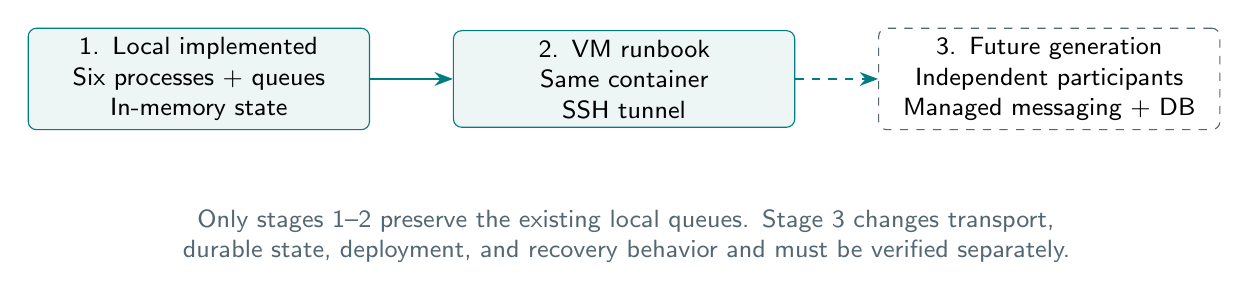
\begin{tikzpicture}[font=\fontsize{9}{11}\selectfont,box/.style={draw=teal,fill=pale,rounded corners=3pt,align=center,text width=4.1cm,minimum height=1.2cm},arr/.style={-{Stealth},thick,teal}]
\node[box] (l) at (0,0) {1. Local implemented\\Six processes + queues\\In-memory state};
\node[box] (v) at (5.4,0) {2. VM runbook\\Same container\\SSH tunnel};
\node[box,draw=muted,dashed,fill=white] (d) at (10.8,0) {3. Future generation\\Independent participants\\Managed messaging + DB};
\draw[arr] (l)--(v);\draw[arr,dashed] (v)--(d);
\node[text=muted,align=center,text width=13.8cm] at (5.4,-2) {Only stages 1--2 preserve the existing local queues. Stage 3 changes transport, durable state, deployment, and recovery behavior and must be verified separately.};
\end{tikzpicture}
\end{center}

\begin{tabularx}{\linewidth}{>{\raggedright\arraybackslash}p{1.8cm}YYY}
\toprule
\textbf{Provider} & \textbf{Participant compute} & \textbf{Transport} & \textbf{Durable state} \\ \midrule
AWS & ECS services & SQS role inboxes & RDS PostgreSQL \\
GCP & Cloud Run services & Pub/Sub topics/subscriptions & Cloud SQL PostgreSQL \\
Azure & Container Apps & Service Bus queues & Azure Database for PostgreSQL \\
\bottomrule
\end{tabularx}
These are proposed mappings, not implemented adapters or provisioned services. A push-service mapping requires a participant HTTP event handler rather than a blocking local queue loop. A worker-service mapping requires a supported pull/long-running execution model.

\smalltitle{Required changes before independent deployment}
\begin{itemize}
\item Replace queue transport behind an explicit send/receive interface; retain stable payment/operation/session IDs.
\item Persist account/hold/batch/fee state and idempotency result atomically. Add a transactional inbox/outbox and retry/dead-letter handling.
\item Authenticate participant traffic and the instructor dashboard; partition sessions explicitly.
\item Establish ordering/concurrency control for accounts and batch membership. Use database transactions and test replay under duplicate/out-of-order delivery.
\item Add recovery/reconciliation, deployment health, logs/traces, cost inventory, and provider-specific teardown.
\end{itemize}

\smalltitle{Bounded generation and verification sequence}
First generate and test a transport interface using an in-memory fake. Next generate one provider adapter and durable issuer operations with fault tests. Then migrate a single role, validate trace/financial invariants, and expand role by role. Preserve the instructor controls through an event-observation API.

Prompt: ``Implement only the selected provider's transport adapter and one durable issuer authorization transaction. Keep existing envelopes and cents. Add duplicate, conflicting-ID, competing-hold, crash-after-write, and redelivery tests. Output deployment manifests for review; do not deploy or claim settlement recovery is complete.''

\clearpage
\pagetitle{20 / TECHNICAL DESIGN}{Sources, artifacts, and maintenance}
\smalltitle{Conceptual and payment sources}
\begin{itemize}
\item Adnan Masood, PhD., \emph{Agentic Payments 101 (1/2): How the Card Payment System Works}, July 11, 2026. User-supplied pasted article; the conceptual starting point, not the simulator's wire specification.
\item \href{https://developer.visa.com/capabilities/visanet-connect-acceptance/docs}{VisaNet Connect -- Acceptance}. Authorization requests reach the issuer and responses return to the client; capture initiates later clearing/settlement. The toy does not call these APIs.
\item \href{https://developer.visa.com/pages/glossary}{Visa developer glossary}. Primary role and payment-stage definitions.
\item \href{https://docs.stripe.com/payments/place-a-hold-on-a-payment-method}{Stripe manual authorization/capture}. A practical example of reserved funds and later capture. Expiry and partial capture described there are outside Project 0.
\end{itemize}

\smalltitle{Runtime and deployment primary sources}
\begin{itemize}
\item \href{https://docs.python.org/3/library/multiprocessing.html}{Python multiprocessing} and \href{https://docs.python.org/3/library/http.server.html}{http.server}: process/context/queue and local HTTP building blocks.
\item \href{https://docs.docker.com/engine/install/ubuntu/}{Docker Engine on Ubuntu}, \href{https://docs.docker.com/reference/cli/docker/image/save/}{docker image save}, \href{https://docs.docker.com/reference/cli/docker/image/load/}{docker image load}, and \href{https://docs.docker.com/reference/cli/docker/container/run/}{docker run}: packaging/transfer and local port publishing.
\item \href{https://docs.aws.amazon.com/lightsail/latest/userguide/getstarted-awscli.html}{AWS Lightsail CLI guide}; command references linked on pages 13--14.
\item \href{https://docs.cloud.google.com/sdk/gcloud/reference/compute/instances/create}{GCP instance creation}, \href{https://docs.cloud.google.com/sdk/gcloud/reference/compute/ssh}{SSH}, \href{https://docs.cloud.google.com/sdk/gcloud/reference/compute/scp}{SCP}, and \href{https://docs.cloud.google.com/solutions/connecting-securely}{secure connections}.
\item \href{https://learn.microsoft.com/en-us/azure/virtual-machines/linux/quick-create-cli}{Azure Linux VM CLI quickstart} and \href{https://learn.microsoft.com/en-us/cli/azure/vm?view=azure-cli-latest}{az vm reference}.
\end{itemize}
Official documentation was checked October 6, 2026. Cloud image IDs, instance sizes, account policies, CLI versions, and prices can change; the runbooks deliberately require provider inventory/permission checks. No cloud resource was provisioned during artifact generation.

\smalltitle{Editable sources and actual screenshots}
Both LaTeX documents define their own style and TikZ diagrams. The technical supplement has no external visual dependencies. The course source optionally loads the real PNGs from \texttt{../screenshots}; keep the distributed directory structure when exporting it. If the source is opened alone in a native standalone editor, bounded fallback panels replace unavailable images. Final package PDFs include the actual captures.

Architecture, sequence, lifecycle, and cloud-evolution diagrams also exist as Mermaid sources and SVG exports in \texttt{docs/diagrams}. Update source and export together if the design changes. The screenshot captures record a real run, so PIDs and times are examples.

\smalltitle{Verification provenance}
Read \texttt{TEST\_REPORT.md and VERIFICATION.json} for executed tests, browser observations, compilation results, page counts, and platform/container limitations. The AI-use record distinguishes generated work and human review needs. The manifest and ZIP make the runnable example portable. Future cloud commands and architecture are an evolution path, not evidence of deployed payment infrastructure.
\end{document}
